\documentclass[10pt,conference]{IEEEtran}
% The preceding line is only needed to identify funding in the first footnote. If that is unneeded, please comment it out.
\usepackage{cite}
\usepackage{amsmath,amssymb,amsfonts}
\usepackage{algorithmic}
\usepackage{graphicx}
\usepackage{textcomp}
\usepackage{xcolor}
\usepackage{fancyhdr}
\usepackage{hyperref}
\usepackage[outputdir=.]{minted}
\usepackage{amsthm}
\usepackage{ragged2e}
\usepackage{mathtools}

\hypersetup{
    colorlinks=true,
    linkcolor=blue,
    filecolor=blue,      
    urlcolor=blue,
    pdftitle={Penerapan Algoritma Decrease and Conquer dalam Mencari Blok Pertama yang Berbeda pada Blockchain},
    pdfpagemode=FullScreen,
}

\urlstyle{same}

\def\abstractname{Abstrak}
\def\IEEEkeywordsname{Kata Kunci}
\def\refname{Daftar Pustaka}

\theoremstyle{definition}
\newtheorem{definition}{Definisi}[section]

\newtheorem{theorem}{Teorema}[section]

\def\BibTeX{{\rm B\kern-.05em{\sc i\kern-.025em b}\kern-.08em
    T\kern-.1667em\lower.7ex\hbox{E}\kern-.125emX}}

\graphicspath{{../img}}

%%% Footer Left
\makeatletter

\def\ps@headings{
\let\@oddhead\@empty
\let\@evenhead\@empty
\def\@oddfoot{Makalah IF2211 Strategi Algoritma – Sem. II Tahun 2021/2022\hfill}
\def\@evenfoot{Makalah IF2211 Strategi Algoritma – Sem. II Tahun 2021/2022\hfill}
}

\def\ps@IEEEtitlepagestyle{% default title page headers, no footers
\let\@oddhead\@empty
\let\@evenhead\@empty
\def\@oddfoot{Makalah IF2211 Strategi Algoritma – Sem. II Tahun 2021/2022\hfill}%
\let\@evenfoot\@empty
}
\makeatother

\pagestyle{headings}

% Document

\begin{document}

\title{Penerapan Algoritma  \emph{Decrease and Conquer} dalam Mencari Blok Pertama yang Berbeda pada Blockchain}

\author{\IEEEauthorblockN{Bayu Samudra - 13520128\textsuperscript{1}}
\IEEEauthorblockA{\textit{Program Studi Teknik Informatika} \\
\textit{Sekolah Teknik Elektro dan Informatika}\\
Institut Teknologi Bandung, Jl. Ganesha 10 Bandung 40132, Indonesia \\
\textsuperscript{1}13520128@std.stei.itb.ac.id}
}

\maketitle

\begin{abstract}
Blockchain merupakan rangkaian blok yang terhubung antara satu dengan lainnya. Blok-blok dalam blockchain dihubungkan dengan mereferensikan nilai hash pada blok sebelumnya. Hash yang digunakan pada makalah kali adalah SHA3. Sifat yang dimiliki algoritma hash ini adalah sangat sensitif terhadap perubahan walaupun kecil. Dengan memanfaatkan sifat ini dan juga struktur blockhain maka dapat dicari blok pertama dari sebuah rantai yang membuat dua buah rantai berbeda. Algoritma ini memanfaatkan pendekatan \emph{decrease and conquer}. Algoritma ini bekerja dalam kompleksitas logaritmik sehingga sangat efisien. Pemanfaatan algoritma ini dapat digunakan pada bidang forensik dan juga keamanan untuk melakukan audit terhadap dua buah blockchain yang berbeda.
\end{abstract}

\begin{IEEEkeywords}
Blockhain, Kriptografi, SHA-32
\end{IEEEkeywords}

\section{Pendahuluan}
Pada saat ini, perkembangan teknologi digital sangatlah berkembang pesat. Banyak sekali teknologi digital yang baru dari tahun ke tahun. Salah satu teknologi yang muncul dan cukup terkenal saat ini adalah mata uang kripto. Mata uang kripto merupakan sebuah aset digital yang dimiliki seseorang dan dilindungi oleh kriptografi untuk menjaga kepemilikan aset tersebut. Mata uang kripto dapat dipertukarkan dari satu mata uang ke mata uang lainnya. Mata uang ini berdiri di atas teknologi blockhain yang saat ini berkembang cukup pesat.

Teknologi blockhain saat ini penggunaanya tidak hanya dipakai untuk mata uang saja. Pemanfaatan lain dari blockchain ini dapat diimplementasikan pada dunia kesehatan, engineering, bahkan hukum. Saat ini berkembang salah satu penerapan blockhain, yaitu \emph{Non-Fungible Token} (NFT) yang berjalan diatas blockhain untuk menjaga kepemilikan dari suatu barang.

Seperti namanya, blockchain terdiri atas beberapa blok yang saling berkaitan satu sama lain. Setiap blok pada blockhain akan diikat dengan referensi hash dari rantai sebelumnya. Oleh karena itu, pengecekan dua buah blok dapat dengan mudah dilakukan dengan cara melihat saja blok terakhir yang disimpan. Selain itu, blok yang  berbeda ini juga dapat dicari dengan berbagai algoritma. Pada makalah kali ini, penulis membatasi pencarian blok yang berbeda hanya pada blok pertama dari sebuah rantai acak yang dibuat.

\section{Teori Dasar}
\subsection{Struktur Blok}
Struktur blok terdiri atas beberapa komponen penting diantaranya adalah sebagai berikut:


    \subsubsection{Hash blok sebelumnya}
    Seperti yang telah diketahui pada bab sebelumnya, blockchain haruslah terdiri dari rangkaian blok yang saling terhubung satu sama lain. Blok ini dihubungkan dengan hash dari setiap blok sebelumnya. Nilai hash ini juga yang akan menjaga integritas dari suatu block dari perubahan. Perubahan terjadi tentu saja akan mengubah nilai hash dari blok tersebut sehingga blok tersebut akan tidak valid.

    \subsubsection{Konten}
    Konten perlu disimpan pada struktur blok. Konten ini dapat berisi data kepemilikan, data transaksi, atau data yang lainnya. Data ini harus terjaga integritasnya sehingga data ini tidak boleh berubah. 

    \subsubsection{Tanda tangan digital} 
    Untuk memastikan otorisasi dari sebuah blok, diperlukan sebuah bukti persetujuan dari blok tersebut. Dalam uang mata kripto, salah satu cara yang dapat dilakukan adalah menyertakan tanda tangan digital dari block tersebut. Tanda tangan digital pada dasarnya merupakan kumpulan bit yang dapat memrepresentasikan keabsahan kepemilikan data berdasarkan kucin privat dan kunci publik. Teknis tanda tangan digital ini akan dijelaskan pada bagian selanjutnya.

    \subsubsection{\emph{Proof of work}} 
    Penjagaan hanya menggunakan hash tentu saja tidaklah cukup. Pengubahan tetap saja dapat  dilakukab dengan cara mengubah isi konten dari data dan juga menghitung ulang seluruh hash dari tiap-tiap blok. Proses perhitungan hash ini biasanya cukup cepat oleh karena itu diperlukan proteksi tambahan yaitu \emph{proof of work}. Proof of work merupakan rangkaian bit yang dapat membuat hash dari sebuah block memiliki pola tertentu. Pencarian rangkaian bit ini tentu saja membutuhkan waktu yang lama sehingga menghambat proses perubahan data pada blockhain.

    
Pada blok yang ideal, seluruh komponen diatas perlu ada. Hal ini untuk menjaga integritas dari blok tersebut dari serangan luar yang tidak diinginkan.

\subsection{Protokol Pengiriman}
Dalam menyebarkan struktur blockchain diperlukan aturan yang dapat menjaga integritas rantai tersebut. Beberapa protokol terinspirasi dari protokol yang diterapkan oleh bitcoin \cite{a2}. Beberapa protokol yang penting adalah sebagai berikut:

\subsubsection{Blok yang ditambahkan valid}
Sebelum sebuah blok ditambahkan pada blockchain, perlu dipastikan blok tersebut harus valid. Blok yang valid dapat didefinisikan sesuai dengan kebutuhan. Salah contoh penerapan validitas pada kasus mata uang kripto adalah setiap blok yang dibuat haruslah cukup dengan jumlah saldo yang dimiliki oleh pengirim.

\subsubsection{Blok baru haruslah ditransmisikan ke seluruh titik}
Setiap blok baru yang dibuat haruslah ditransmisikan ke seluruh pemirsa yang berada pada jaringan. Hal ini untuk menjaga keaslian dari rantai blok yang telah dibentuk dikarenakan rangkaian yang asli tersebar di seluruh komputer  yang berada pada jaringan. Untuk mengubah rantai, siperlukan mengubah semua rantai yang ada pada jaringan.

\subsubsection{Blok yang akan ditambahkan haruslah berasal dari rantai yang valid}
Disini rantai yang valid didefinisikan rantai yang tersusun atas blok-blok yang valid. Keabsahan dari rantai dapat dilihat dari rantai terakhir pada sebuah blok. Apabila hash terakhir tertera pada blok yang akan ditambahkan dan blok yang akan ditambahkan sah, rantai tersebut bisa jadi valid. Untuk pemeriksaan terakhir, perlu dilakukan sampling dari node lain apakah rantai yang dimiliki saat ini valid. Hal ini dapat dilakukan pemeriksaan juga menggunakan blok  terakhir. Bila terjadi perbedaan, dapat dilakukan perubahan sesuai dengan rantai yang benar yang berasal dari node lain.

\subsection{Pembangkit Bilangan Acak}
Pembangkit bilangan acak merupakan salah satu alat penting dalam kriptografi. Pembangkit bilangan acak ini akan dibutuhkan dalam beberapa algoritma kriptografi. Terdapat beberapa algoritma pembangkit bilangan acak yang tersedia diantaranya adalah sebagai berikut:

\subsubsection{Linear Congruential Generator (LCG)}

Pembangkit bilangan acak ini didasarkan pada rekursifitas terhadap nilai sebelumnya. Berdasarkan sumber dari \cite{b1}, Berikut ini adalah formula yang dapat digunakan untuk mendapatkan nilai acak menggunakan LCG:

\begin{equation} \label{eq:lcg}
    x_{i+1} = (ax_i + b) \mod m
\end{equation}

Untuk memulai pembangkitan bilangan acak, diperlukan nilai $x_0$ yang merupakan umpan dari bilangan acak ini.

Periode bilangan acak dari LCG ini pastilah tidak akan melebihi nilai $m$. Hal ini dikarenakan adanya modulo yang diberikan pada persamaan \ref{eq:lcg}. Menurut \cite{a1}, Algoritma ini memiliki periode sebagai berikut:

\begin{theorem}[Teorema Hull–Dobell] \label{theo:hulldobell}
    Sebuah LCG yang didefinisikan pada definisi \ref{eq:lcg} dapat memiliki periode penuh, yaitu berperiode $m-1$ jika memenuhi syarat berikut:
    \begin{enumerate}
        \item $b$ relatif prima terhadap $m$,
        \item $a \equiv 1 \text{(mod }p\text{)}$ jika $p$ merupakan faktor prima dari $m$,
        \item $a \equiv 1 \text{(mod }4\text{)}$ jika $m$ adalah bilangan yang habis dibagi oleh 4.
    \end{enumerate}
\end{theorem}

Pembangkit bilangan acak berbasis LCG biasanya sudah tersedia  dalam berbagai bahasa pemrograman. Selain mudah diimplementasikan, algoritma ini juga sangat mangkus dikarenakan hanya diperlukan kompleksitas $O(1)$ dalam membuat bilangan acak. Sayangnya, algoritma ini cukup mudah ditebak nilai acaknya sehingga tidak cocok untuk penggunaan kriptografi. \cite{b1}

\subsubsection{Blum-Blum-Shub}

Algoritma \emph{Blum-Blum-Shub} (BBS) merupakan salah satu algoritma pembangkit bilangan acak yang lebih aman untuk kebutuhan kriptografi. Menurut \cite{b1}, algoritma ini merupakan algoritma yang paling mangkus dan paling seerhana dari semua algoritma pembangkitan bilangan acak yang termasuk dalam kategori \emph{cryptographically-secure pseudorandom number generator} (CSPRNG). Menurut \cite{b1}, Berikut ini adalah algortma yang digunakan untuk membuat bilangan acak menggunakan BBS:

\begin{enumerate}
    \item Menentukan bilangan prima rahasia $p$ dan $q$ yang memenuhi kongruensi berikut

    \begin{equation} \label{eq:bbs1}
        p \equiv q \equiv -1 \text{ }(\text{mod } 4) 
    \end{equation}
    \item Hitunglah nilai $n = pq$. Nilai $n$ ini disebut dengan bilangan bulat blum. 
    \item Diperlukan menentukan nilai umpan $x_0$. Untuk mendapatkan nilai ini, tentukan bilangan bulat acak lain, misalkan $s$ yang memenuhi:
    \subitem $1 < s < n$
    \subitem $s$ dan $n$ relatif prima.

    Nilai $x_0$ dengan formula sebagai berikut 
    \begin{equation} \label{eq:bbs2}
        x_0 = s^2 \mod n
    \end{equation}
    \item Nilai $x_i$ bisa diperoleh dengan formula berikut
    \begin{equation} \label{eq:bbs3}
        x_i = x_{i-1}^2 \mod n
    \end{equation}
    \item Diambil nilai LSB dari $x_i$ sebut saja $z_i$. Nilai $z_i = x_i \mod 2$. Nilai $z_i$ menyusun bit-bit dari bilangan baru yang dibentuk.
\end{enumerate}

\subsection{SHA-3 (Keccak)}
SHA-3 meupakan algortma fungsi hash satu arah yang dibuat oleh Guido Breton, Joan Daemen, dan Michaël Peeters. Algoritma ini menggantikan algoritma MD5 dan SHA-1 yang telah ditemukan kolisinya sehingga sudah tidak aman lagi.

Menurut \cite{b1},  Fungsi hash merupakan fungsi yang menerima masukan string dengan panjang sembarang dan menghasilkan hash yang memiliki panjang tetap. Fungsi hash satu arah berarti pesan yang telah melakukan kompresi menjadi nilai hash tidak bisa dipulihkan kembali menjadi nilai aslinya.

Berdasarkan \cite{b1}, Dalam algoritma SHA-3 dikenal sebuah istilah spons. Spons merupakan state yang diinisialisasi dengan nilai 0. Pada algoritma ini dikenal beberapa fase, yaitu sebagai berikut: 

\begin{enumerate}
    \item Fase Persiapan \\
    Pada fase ini, pesan yang akan dihash akan diberikan padding terlebih dahulu dan dipecah menjadi beberapa blok dengan ukuran $r$. 
    \item Fase Penyerapan \\
    Pada fase ini, blok-blok yang telah dipecah tadi diserap dengan cara melakukan operasi xor terhadap spons dengan panjang $r$. Hasil operasi tersebut lalu dimasukan ke dalam fungsi permutasi. Hal ini dilakukan hingga semua blok sudah terisi.
    \item Fase Pemerasan \\
    DIlakukan inisialisasi pada string kosong $Z$. Selagi panjang $Z$ belum sama dengan panjang string keluaran yang diinginkan, ambil $r$ digit pertama disambungkan dengan $Z$ lalu masukan spons ke dalam fungsi permutasi.   
\end{enumerate}

Berikut ini adalah ilustrasi pembentukan spons dari algoritma SHA-3.

\begin{figure}[htbp]
    \centerline{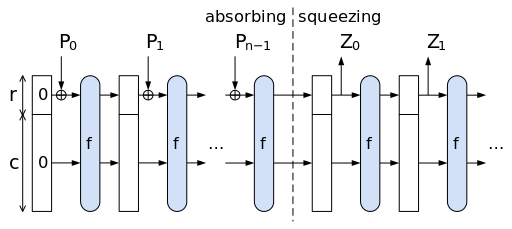
\includegraphics[width=0.9\columnwidth]{fig1.png}}
    \caption{Ilustrasi pembentukan spons (Sumber: Wikipedia)}
\end{figure}

\subsection{Digital Signature Algorithm (DSA)}
Salah satu aspek penting yang harus ada dalam blockhain adalah tanda tangan digital. Terdapat cukup banyak algoritma tanda tangan digital yang teredia. Untuk bahasan kali ini, penulis hanya membatasi membahas mengenai tanda tangan digital DSA (\emph{Digital Signature Algorithm}).

Dikutip dari \cite{b1}, Sebelum melakukan proses diperlukan melakukan perhitungan beberapa nilai sebagai berikut: 
\begin{itemize}
    \item Nilai $p$ merupakan bilangan prima yang bersifat publik dengan panjang $L$.  Nilai $L$ haruslah kelipatan 64 dan berada pada rentang $64 \le L \le 1024$. 
    \item Nilai $q$ merupakan bilangan prima 160 bit yang merupakan faktor dari $p - 1$ dan bersifat publik.
    \item Nilai $g = h ^ {(p-1)/q}$ dengan nilai $h < p - 1$ sehingga membuat nilai $g \mod p > 1$. Nilai ini bersifat publik.
    \item $x$ merupakan bilangan bulat kurang dari $q$.  Nilai ini bersifat privat.
    \item Nilai $y = g^x \mod p$ yang merupakan kunci publik.
    \item Pesan $M$ yang akan ditandatangani.
    \item Nilai $H(M)$ yang merupakan hash dari pesan $M$.
\end{itemize}

Untuk membuat tanda tangan, seorang pengirim perlu mendapatkan sebuah angka acak $k$ yang kurang dari $q$. Tanda tangan $r$ dan $s$ dapat didapatkan dengan rumus sebagai berikut: \cite{b1}

\begin{equation} \label{eq:dsa1} 
    r = (g^k \text{ mod } p) \text{ mod } q
\end{equation}

\begin{equation} \label{eq:dsa2} 
    s = k^{-1}(H(M) + xr) \text{ mod } q
\end{equation}

Untuk melakukan verifikasi pesan, seorang penerima perlu mendapatkan nilai $(p,q,g,y)$ dan hasil tandatangan $(r,s)$. Perhitungan yang dilakukan adalah sebagai berikut: \cite{b1}

\begin{equation} \label{eq:dsa3} 
    w = s^{-1} \text{ mod } q
\end{equation}
\begin{equation} \label{eq:dsa4} 
    u_1 = (H(M) \cdot w) \text{ mod } q
\end{equation}

\begin{equation} \label{eq:dsa5} 
    u_2 = rw \text{ mod } q
\end{equation}

\begin{equation} \label{eq:dsa6} 
    v = ((g^{u_1} \cdot y^{u_2}) \text{ mod } p) \text{ mod } q
\end{equation}

Apabila nilai $v = r$, dapat dikatakan tandatangan sah.

\subsection{Decrease and Conquer (DnC)}

\emph{Decrease and conquer} (DnC) merupakan metode perancangan algoritma penyeselaian dengan mereduksi persoalan menjadi dua bagian yang selanjutnya akan dipilih sebuah sub persoalan untuk dievaluasi selanjutnya. \cite{ppt1}

Terdapat beberapa variasi dari metode \emph{Decrease and conquer}, yaitu sebagai berikut

\begin{itemize}
    \item \emph{Decrease by constant} \\
    Pada variasi ini, ukuran persoalan dikurangi berdasarkan besar yang konstan setiap iterasi algoritma berlangsung. Salah satu contoh algoritma yang termasuk dalam kategori ini adalah \emph{selection sort} dengan konstanta 1.
    \item \emph{Decrease by constant factor} \\
    Pada variasi ini, ukuran persoalan direduksi berdasarkan nilai faktor yang konstan selama iterasi berlangsung. Salah satu contoh algoritma yang termasuk dalam kategori ini adalah pencarian biner dengan faktor konstanta 2.
    \item \emph{Decrease by variable size} \\
    Pada variasi ini, ukuran persoalan direduksi dengan jumlah bervariasi setiap kali dilakukannya iterasi.  Salah satu contoh algoritma yang termasuk dalam bentuk ini adalah pencarian interpolasi.
\end{itemize}

Algoritma ini juga terdiri atas dua tahapan penting yaitu sebagai berikut:
\begin{enumerate}
    \item \emph{Decrease} \\
    Pada tahap ini, persoalan  akan dibagi menjadi beberapa upa-persoalan yang lebih kecil.
    \item \emph{Conquer} \\
    Pada tahap ini, akan dipilih sebuah upa-persoalan yang akan diselesaikan. Upa-persoalan terpilih akan diselesaikan kembali menggunakan DnC secara  rekursif.
\end{enumerate}

\section{Perancangan Algoritma}

Pada bab ini, akan dibahas rancangan algoritma yang digunakan untuk menyelesaikan permasalahan.

\subsection{Deskripsi Permasalahan}
Akan dibandingkan kesamaan antara dua buah blockchain yang sama panjang. Bila kedua blockchain berbeda, akan dicari blok pertama yang menyebabkan kedua blockchain berbeda. 

\subsection{Asumsi dan Batasan}
Dalam perancangan ini, diberikan beberapa asumsi sebagai berikut:
\begin{itemize}
    \item Blockhain bisa saja memiliki lebih dari 1 buah blok yang berbeda.
    \item Nilai hash dari blok sebelumnya valid. Hal ini berarti tidak ada blok yang memiliki nilai blok yang berbeda dengan yang dicatatkan pada blok tersebut.
    \item Dalam pengujian, struktur blockhain hanya terdiri atas nilai hash sebelumnya dan konten dari blok. Hal ini dimaksudkan untuk menyederhanakan dan mempercepat proses pengujian.
\end{itemize}

\subsection{Desain Algoritma}
Algoritma yang digunakan menggunakan metode \emph{decrease and conquer} berbasis \emph{decrease by constant factor}. Faktor yang  digunakan untuk mereduksi adalah 2. Berikut ini adalah algoritma lengkap mengenai proses yang dilakukan saat pencarian blok yang berbeda:

\begin{enumerate}
    \item Set nilai awal $l$ sebagai indeks batas bawah (inklusif) dari pencarian dan nilai $r$ sebagai indeks batas atas (eksklusif) dari pencarian.
    \item Cek apakah nilai $l < r$. Bila tidak hentikan iterasi. Kedua blockchain merupakan blok yang sama.
    \item Hitung hash blok tengah dengan indeks ke-$\lfloor \frac{l+r}{2} \rfloor$ dari kedua blok.
    \item Bila nilai hash dari keduanya sama, maka set nilai $l$ menjadi $\lfloor \frac{l+r}{2} \rfloor$. Lanjutkan iterasi ke langkah ke-2.
    \item Bila nilai hash dari keduanya tidak sama, perlu diperiksa letak dari blok tengah. Bila blok tengah merupakan blok awal (berindeks 0), maka kedua blockchain berbeda pada blok pertama. Hentikan iterasi.
    \item Bila nilai hash dari keduanya tidak sama dan blok tengah tidak berada pada indeks 0, perlu diperiksa hash blok sebelumnya. Apabila hash blok sebelumnya dari kedua blockchain memiliki nilai yang sama, blok pertama yang berbeda adalah blok tengah. Hentikan iterasi.
    \item Bila nilai hash dari keduanya tidak sama , blok tengah tidak berada pada indeks 0, dan indeks sebelumnya berbeda, ubah nilai $r$ menjadi $\lfloor \frac{l+r}{2} \rfloor$. Lanjutkan iterasi ke langkah 2.
\end{enumerate}

\subsection{Psedeocode Penyelesaian}
Psedeocode dari penyelesaian permasalahan di atas ditunjukan oleh algortma pada figur \ref{algo:1}.


\begin{figure}
    \begin{minted}{go}
func FindFirstDiff(chain1, chain2 Chain) 
    int64 {
  if chain1.length != chain2.length {
      panic("Ukuran chain harus sama")
  }
  
  l := int64(0)
  r := chain1.length
  
  for l < r {
      center := (l + r) / 2
      diff := 
        CheckDifference(chain1, chain2, 
          center)
  
      if diff == 0 {
        return center
      } else if diff > 0 {
        l = center + 1
      } else {
        r = center
      }
  }
  
  return -1
}
        
    \end{minted}
    \caption{Algoritma Pencarian Blok dengan DnC}
    \label{algo:1} 
\end{figure}

Fungsi CheckDifference() memberikan nilai 0 pada saat ditemukan blok yang berada pada indeks ke-0 tapi berbeda atau blok yang tidak berada di indeks ke-0, berbeda, dan hash sebelumnya sama. Fungsi ini juga memberikan nilai 1 apabila ditemukan nilai blok yang dites pada indeks tersebut sama. Fungsi ini juga memberikan nilai -1 bila blok pada indeks yang dipilih dan pada indeks sebelumnya dari dua buah blockchain berbeda.


\begin{figure}
    \begin{minted}{go}
func CheckDifference(Chain1, Chain2 Chain,
    idx int64) int64 {
  it1 := Chain1.GetChainItem(idx)
  it2 := Chain2.GetChainItem(idx)
  
  if it1.GetBase64Hash() 
     != it2.GetBase64Hash() {
    if idx > 0 {
      last1 := Chain1.GetChainItem(idx - 1)
      last2 := Chain2.GetChainItem(idx - 1)
  
      if last1.GetBase64Hash() == 
        last2.GetBase64Hash() {
        return 0
      } else {
        return -1
      }
    } else {
      return 0
    }
  } else {
    return 1
  }
}        
    \end{minted}
    \caption{Algoritma Pembanding}
    \label{algo:2} 
\end{figure}

Nilai 0 pada fungsi CheckDifference() berarti blok yang membuat dua buah chain berbeda ditemukan. Nilai -1 berarti blok yang membuat berbeda berada pada indeks kurang dari indeks saat ini. Nilai 1 berarti blok yang  membuat berbeda bisa jadi berada pada indeks yang lebih besar dari indeks saat ini. Pemberian nilai 1 pada fungsi ini tidak menjamin akan mendapatkan blok yang berbeda dikarenakan bisa jadi kedua buah blockchain sama.

\subsection{Analisis Kompleksitas}
Berdasarkan algoritma yang telah dipaparkan sebelumnya, terlihat bahwa permasalahan akan tereduksi menjadi dua seiring waktu secara rekursif. Diasumsikan perhitungan kompleksitas berdasarkan jumlah perbandingan yang terjadi. Berikut ini adalah kompleksitas waktu yang ditbutuhkan oleh algoritma:

$$ 
T(n) =
\begin{cases}
    1, &\text{jika } n = 0\\
    T(n/2) + 2, &\text{sisanya}
\end{cases}
$$

Perbandingan terjadi saat pengecekan kondisi kalang dan juga pengecekan nilai tengah. Dari nilai diatas, dapat disimpulkan bahwa notasi big-O dari algoritma ini adalah sebagai berikut:

$$
T(n) = O(\log n)
$$

\subsection{Analisis Solusi}
Proses penyelesaian ini mirip dengan proses pencarian biner. Hal ini bisa dilakukan dikarenakan sifat dari nilai hash itu sendiri. Seperti yang telah diketahui sebelumnya, nilai hash berubah cukup jauh walaupun perubahan yang terjadi cukup kecil. Hal ini bisa berdampak pada rantai selanjutnya apabila terdapat perbedaan nilai hash.

Ilustrasi dari proses ini, misalkan terdapat dua rantai dengan panjang $n$. Rantai ini memiliki pesan blok yang berbeda pada indeks ke-$k$. Nilai hash pada indeks ke-0 sampai dengan indeks ke-$(k-1)$ pastilah memiliki nilai yang sama. Hal ini dikarenakan konten data yang dilibatkan pada rantai ini sama. 

Pada blok ke-$k$, terjadi perbedaan konten dari blok tersebut. Disini akan muncul perbedaan hash dari kedua buah blockhain. Dikarenakan setiap blok mereferensikan hash blok sebelumnya, nilai hash blok setelah indeks ke-$k$ bisa berbeda cukup signifikan dibandingkan dengan blok pada blockhain lainnya. 

Proses pencarian ini dilakukan dengan memeriksa blok tengah dari rantai yang akan diperiksa. Misal saja blok tersebut berada di indeks ke-$i$. Apabila blok indeks ke-$i$ memiliki nilai hash yang sama, blok pada indeks kurang dari $i$ tentu saja dapat dipastikan sama. Oleh karena itu, proses pemeriksaan dapat dilanjutkan dengan memindahkan awal pencarian ke indeks $i+1$. Proses ini dapat mengurangi pemeriksaan yang diperlukan.

Apabila pada saat pemeriksaan di indeks ke-$i$ didapati terjadi perbedaan nilai hash, dapat terjadi dua buah kemungkinan. Kemungkinan pertama, apabila indeks ke-$i$ merupakan blok yang paling pertama ($i=0$), dapat  dipastikan blok tersebut adalah blok pertama yang menyebabkan kedua rantai tersebut berbeda.

Berbeda halnya bila blok pada indeks ke-$i$ bukan merupakan blok awal. Diperlukan untuk melakukan pemeriksaan terlebih dahulu pada blok sebelumnya, yaitu blok dengan indeks ke-$(k-1)$. Apabila didapati blok dengan indeks ke-$(k-1)$ memiliki nilai hash yang sama pada kedua rantai, dapat dipastikan bahwa blok dengan indeks dari 0 sampai dengan indeks ke-$(k-1)$ sama. Oleh karena itu, pastilah blok pada indeks ke-$k$ merupakan blok pertama yang menyebabkan terjadinya perbedaan antara kedua rantai.

Apabila kedua buah rantai memiliki nilai hash yang berbeda pada indeks ke-$(k-1)$, tidak dapat dipastikan blok pada indeks ke-$(k-1)$ merupakan blok yang pertama kali menyebabkan kedua buah rantai ini berbeda. Akan tetapi, dapat dipastikan blok yang menyebabkan rantai berbeda pertama kali berada pada indeks kurang dari $k$. Hal ini terlacak dari perbedaan pada nilai hash indeks ke-$k$ dan juga indeks ke-$(k-1)$ yang keduanya sama-sama berbeda. Oleh karena itu, perlu dilakukan pencarian dari indeks ke-$0$ sampai dengan indeks ke-$(k-1)$.

Dari penjelasan diatas dapat terlihat, pada saat pemeriksaan suatu blok indeks ke-$k$ terjadi perbedaan nilai hash, dapat dipastikan terdapat paling tidak satu buah blok yang berbeda pada indeks ke-0 sampai dengan indeks ke-$(k-1)$. Namun, apabila nilai hash pada indeks ke-$k$ memiliki nilai yang sama, belum bisa dipastikan akan terdapat sebuah blok pada indeks lebih dari $k$ yang menyebabkan dua buah blockchain berbeda.

\section{Pengujian Solusi}
Pada bagian ini, akan dilakukan pengujian solusi yang telah ditawarkan pada bagian sebelumnya. 

\subsection{Teknis Pengujian}
Pengujian akan dilakukan dengan membandingkan solusi yang dihasilkan dengan algoritma yang dipaparkan diatas dengan algoritma penyelesaian secara brute force. Selain itu, akan dilakukan perhitungan waktu eksekusi tiap-tiap uji kasus. Uji kasus akan dibuat secara acak dengan ukuran konten maksimal 1024 bytes. Panjang rantai yang akan dipakai dalam pengujian adalah antara 1000 s.d. 100.000. (Inklusif) sebanyak 45 data.

\subsection{Hasil Pengujian}

Berikut ini adalah ringkasan data hasil pengujian yang dilakukan.
\vspace{8px}

\begin{tabular}{|l|l|l|}
\hline
\textbf{Data Statistik} & \textbf{Waktu Brute Force} & \textbf{Waktu DnC} \\ \hline
Rata-rata               & 0,23 s                     & 168 us             \\ \hline
Standar Deviasi         & 0.2 s                      & 56 us              \\ \hline
Maksimum                & 0.7 s                      & 328 us             \\ \hline
Minimum                 & 0.5 ms                     & 60 us              \\ \hline
\end{tabular}

\vspace{8px}

Grafik hasil pengujian ditunjukan pada gambar \ref{fig:grafik}. Pada grafik tersebut, titik biru menyatakan waktu eksekusi saat menggunakan algoritma \emph{Brute Force}. Titik berwarna jingga merupakan waktu eksekusi saat menggunakan algoritma  \emph{decrease and conquer}.

\begin{figure}[htbp]
    \centerline{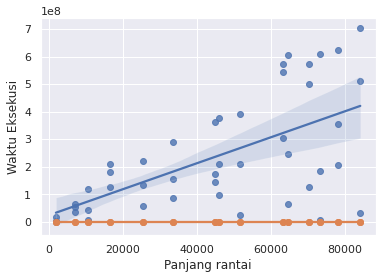
\includegraphics[width=0.9\columnwidth]{grafik.png}}
    \caption{Waktu Eksekusi}
    \label{fig:grafik}
\end{figure}

Hasil yang dikeluarkan oleh algoritma secara \emph{Brute Force}  dan \emph{decrease and conquer} semuanya sama. Hal ini terlihat dari berbagai sampel dengan ukuran rantai acak, tidak ditemukan perbedaan hasil.


\subsection{Analisis Hasil Pengujian}
Dari hasil pengujian di atas terlihat bahwa waktu eksekusi menggunakan \emph{Brute Force} jauh lebih besar dibangkan dengan waktu eksekusi menggunakan \emph{decrease and conquer}. Hal ini dibuktikan dengan garis biru yang lebih cepat untuk menaik dibandingkan denggan garis jingga yang lebih lambat untuk menaik. Hal ini terjadi dikarenakan kompleksitas algoritma \emph{brute force} berada pada tingkat $O(n)$. Hal ini cukup jauh signifikan dengan algoritma \emph{decrease and conquer} yang memiliki kompleksitas $O(\log n)$, 

Selain itu, belum ditemukan kasus yang menyebabkan hasil dari kedua algoritma ini berbeda. Oleh karena itu, algoritma ini dapat digunakan untuk melakukan pencarian indeks blok pertama yang menyebabkan kedua blockchain berbeda.

\section{Kesimpulan}
Blockchain merupakan salah satu teknologi yang dapat menjaga integritas data walaupun data disebarkan secara publik. Blockchain ini dapat dimanfaatkan dalam berbagai bidang. Blockchain pada dasarnya terdiri atas blok-blok yang saling terhubung satu sama lain. Satu blok terhubung dengan blok sebelumnya dengan cara mereferensikan nilai hash dari blok sebelumnya pada blok baru.

SHA-3 merupakan hash satu arah bersifat \emph{irreversible} dan juga sangat sensitif dengan perubahan kecil. Pemanfaatan fungsi hash ini akan melindungi dari perubahan yang terjadi. 

Dengan keterhubungan tersebut, dapat digunakan algoritma yang telah dipaparkan sebelumnya untuk mencari blok yang memiliki nilai berbeda. Algortma ini juga memiliki kompleksitas yang cukup memuaskan yaitu $O(\log n)$.

Pemanfaatan algoritma ini dapat digunakan oleh tim forensik untuk mengaudit sebuah blockchain panjang. Pengauditan ini dapat dipakai untuk memeriksa manakah penyebab blockchain berbeda dan menganalisis informasi pesan yang terkandung dalam blockchain tersebut. 

\section*{Ucapan Terima Kasih}
Alhamdulillah, segala puji Allah SWT karena atas pertolongan, rahmat, serta hidayahnya, saya dapat menyelesaikan makalah ini. Sholawat serta salam semoga selalu tercurahkan kepada Nabi Muhammad SAW yang telah memberikan jalan lurus menuju kebenaran. 

Penulis memberikan ucapan terima kasih kepada keluarga yang selalu setia untuk
memberikan motivasi dan semangat untuk dapat menyelesaikan makalah ini. Penulis juga turut mengucapkan terima kasih kepada para dosen pengampu mata kuliah Matematika Diskrit, yaitu ibu Dr. Nur Ulfa Maulidevi, S.T., M.Sc., bapak Dr. Ir.
Rinaldi Munir, M.T., dan ibu Dr. Masayu Leylia Khodra. atas segala ilmunya yang telah membantu penulis dalam menyelesaikan makalah ini. Penulis juga turut berterima kasih kepada sahabat saya, Hana Fathiyah, yang selalu setia menemani dalam berbagai keadaan. Semoga dengan kebaikan yang telah diberikan, Allah akan menggantinya dengan yang lebih baik lagi.

\section*{Sumber Daya}
Segala sumber daya yang digunakan untuk membangun makalah ini dapat anda akses pada \url{https://github.com/bayusamudra5502/stima-blockchain}.


\begin{thebibliography}{00}
\bibitem{b1} Munir, Rinaldi. 2019. \emph{Kriptografi Edisi Kedua}. Bandung: Penerbit Informatika 
\bibitem{ppt1} Munir, Rinaldi. 2021. Algoritma Decrease and COnquer. Bandung: Institut Teknologi Bandung. DIakses pada 2022-05-21 melalui https://informatika.stei.itb.ac.id/~rinaldi.munir/Stmik/2020-2021/Algoritma-Decrease-and-Conquer-2021-Bagian1.pdf
\bibitem{a1} Hull, T. E. \& Dobell, A. R. 1962. Random Number Generators. SIAM Review, 4(3), 233. Diakses pada 2022-05-21 melalui http://chagall.med.cornell.edu/BioinfoCourse/PDFs/Lecture4\\
/random\_number\_generator.pdf.
\bibitem{a2} Nakamoto, Satoshi. 2008. Bitcoin: A Peer-to-Peer Electronic Cash System. Diakses pada 2022-05-21 melalui https://bitcoin.org/bitcoin.pdf.
\end{thebibliography}

\section*{Pernyataan}
Dengan ini saya menyatakan bahwa makalah yang saya tulis adalah tulisan saya sendiri, bukan sanduran, ataupun terjemahan dari makalah orang lain, dan bukan plagiasi.


\vspace{20px}
\hspace*{\fill} Cimahi, 21 Mei 2022

\vspace{50px}
\hspace*{\fill} Bayu Samudra - 13520128

\end{document}
